\section{基于物理的渲染简史}\label{sec:基于物理的渲染简史}

20世纪70年代早期计算机图形学中,
最重要的问题是解决可见性算法和几何表示等基础问题。
那时兆字节的RAM还是稀有昂贵的奢侈品,
每秒能执行百万次浮点运算的计算机要花费数十万美元,
因此计算机图形学中能达到的复杂度也相应受限,
任何为了渲染而尝试精确模拟物理的做法都不切实际。

随着计算机越来越强大和廉价,
考虑计算需求更大的渲染方法成为可能,
这也让基于物理的方法变得可行。
\keyindex{布林定律}{Blinn's law}{}简洁地解释了这一过程:
“随着技术进步,渲染时间保持不变。”

Jim Blinn简单的表述抓住了一条重要的约束:
给定某数量必须要渲染的图像
(对研究论文可能是几张,对故事片则超过十万张),
每张只可能花费这么多处理时间。
有人只有特定数量的计算资源,
有人必须在特定时间内完成渲染,
因此有必要限制每张图像的最大计算量。

布林定律也点明了一个现象:
人们想要渲染的图像和他们能渲染的图像还存在差距:
随着计算机越来越快,
内容创作者会持续利用增加的计算能力
和更精巧的渲染算法渲染更复杂的场景,
而不只是更快地渲染和以前一样的场景。
渲染会持续消耗其可用的全部计算力。

\subsection{研究}\label{sub:研究}
20世纪80年代图形学研究者开始认真考虑基于物理的渲染方法。
\citet{10.1145/358876.358882}的论文介绍了
为全局光照效果使用光线追踪的思想,
打开了精确模拟场景中光分布的大门。
其产生的渲染图像与以前的明显不同,
让人兴奋不已。

基于物理的渲染中另一个值得注意的早期进步是
\citet{10.1145/800224.806819}与\citet{10.1145/357290.357293}的反射模型,
将微面反射\sidenote{译者注:原文microfacet reflection。}模型引入图形学。
除其他贡献外,他们证明
对微面反射精确建模能做到精确渲染金属表面;
更早方法无法很好地渲染金属。

不久后,\citet{10.1145/800031.808601}将热传递文献与渲染联系起来,
展示了如何利用基于物理的光传输近似加入全局漫射\sidenote{译者注:原文diffuse。}光效果。
该方法基于有限元\sidenote{译者注:原文finite-element。}方法,
场景中表面区域互换能量。
在有相关物理单位后,该方法称为“光能传递”
\sidenote{译者注:原文radiosity,有光能传递、辐射着色、辐射度等含义。
    此处按上下文暂译为光能传递。}。
\citet{10.1145/325334.325171}以及
\citet{10.1145/325334.325169}的后续工作引入了重要改进。
基于物理的方法再次得到了在以前的渲染图像中从未见过的带有光照特效的图像,
带动了许多研究者在这一领域竞相提升。

尽管光能传递方法主要基于物理单位和能量守恒,
但随着时间推移它不能得到可行渲染算法的事实越来越明显:
其渐进复杂度是难以控制的$O(n^2)$,
且需要能够沿阴影边界再细分\sidenote{译者注:原文re-tessellate。}几何模型以获得好的结果;
研究者为这个目的开发出稳定高效的细分算法是很困难的,
光能传递在实际应用中受到限制。

在光能传递的年代,一小部分研究者追求
基于光线追踪和蒙特卡洛积分的基于物理的渲染方法。
那时许多人对他们的工作持怀疑态度;
蒙特卡洛积分的变化在图像中引起令人讨厌的噪声似乎是不可避免的,
而基于光能传递的方法至少在相对简单的场景上能快速给出视觉上讨喜的结果。

1984年,\citet{10.1145/800031.808590}引入了分布式光线追踪,
将Whitted的算法推广到从相机计算运动模糊和散焦模糊、
来自光泽表面的模糊反射以及来自面光源的照明,
表明光线追踪能生成众多重要的光照效果。

之后不久,\citet{10.1145/15922.15902}引入了路径追踪;
他提出渲染问题的严格公式(光传输方程)
并说明如何用蒙特卡洛积分求解它。
这需要大量计算:
用路径追踪渲染一幅有两个球体的$256\times256$像素图像
需要一台IBM 4341计算机运行7小时,
其首次发布花了约280,000美元\citep{farmer1981comparing}。
\citet{10.1145/800031.808594}
也把体积渲染方程引入了图形学;
该方程严格描述了介质中的光散射。

Cook等和Kajiya的工作都再次得到了前所未见的图像,
证明了基于物理方法的价值。
随后几年,\citet{10.1145/97879.97886}与
\citet{10.1145/122718.122735}的论文
描述了关于蒙特卡洛合成逼真图像的重要工作。
\citet{10.5555/124947}的博士论文和
后续\citet{10.1145/226150.226151}的工作
也对基于蒙特卡洛的方法做出重要贡献。
\citet{10.1007/978-1-4612-3526-2}的《\citetitle{10.1007/978-1-4612-3526-2}》是
最早基于物理框架论述渲染的著作之一,
\citet{GLASSNER1995}的《\citetitle{GLASSNER1995}》严格
奠定了该领域的基础。
\citet{10.1145/192161.192286}的\emph{Radiance}渲染系统
是早期基于物理的开源渲染系统,专注光照设计,
\citet{slusallek1996vision}的\emph{Vision}渲染器专门缩小基于物理的方法
与当时流行的不基于物理的\emph{RenderMan}接口的差距。

继Torrance和Cook后,
康奈尔大学计算机图形学计划的
许多研究调研了基于物理的方法。
\citet{10.1145/258734.258914}总结了这些工作的动机,
基于真实世界材料属性的度量和对人类视觉系统的深刻理解,
他们强烈支持物理精确渲染。

\citet{veach1997robust}的工作使基于物理的渲染迈出关键一步,
他的博士论文对此进行了详细描述。
\citeauthor{veach1997robust}改进了蒙特卡洛渲染的关键理论基础
还开发了多重要性采样\sidenote{译者注:原文multiple importance sampling。}、
双向路径追踪和Metropolis光传输等新算法,极大提高了效率。
以布林定律为指导,我们认为显著提升的效率对这些方法的实际应用至关重要。

大约这时,随着计算机变得更快更并行化,
许多研究者开始追求实时光线追踪;
\citet{10.1007/978-3-7091-6242-2_26}写了
一篇很有影响力的论文,描述了一个
比以往的光线追踪器高效得多的高度优化的光线追踪器。
许多后续论文介绍了越来越高效的光线追踪算法。
尽管这些工作大多数都不是基于物理的,
但其结果让光线追踪加速结构和光线追踪几何部分的性能有了巨大进步。
因为基于物理的渲染一般大量使用光线追踪,
所以这项工作反过来也带来了和更快的计算机相同的好处,
使得用物理方法能够渲染更复杂的场景。

至此,基于物理的渲染研究进展中关键步骤的总结就介绍到这儿;
还有许多工作没提到。
本书所有后续章节的“扩展阅读”部分将会详细介绍这些工作。

\subsection{制作}\label{sub:制作}
随着20世纪80年代出现更强大的计算机,计算机图形学开始用于动画和电影制作。
早期例子包括Jim Blinn渲染的旅行者2号
\sidenote{译者注:即Voyager 2,于1977年8月20日在肯尼迪航天中心成功发射升空。}
在1981年飞掠土星\sidenote{译者注:在线观看\url{https://youtu.be/SQk7AFe13CY}。}
和电影《星际旅行2:可汗怒吼》\sidenote{译者注:Star Trek II: The Wrath of Khan。}(1982)、
《电子世界争霸战》\sidenote{译者注:Tron。}(1982)以及
《最后的星空战士》\sidenote{译者注:The Last Starfighter。}(1984)中的视觉效果。

在早期运用计算机合成影像进行制作中,
基于栅格化\sidenote{译者注:原文rasterization-based。}的渲染
(尤其是Reyes算法\citep{10.1145/37401.37414})是唯一可行的选项。
一个原因是没有足够的计算力支持基于物理的光线追踪提供的复杂反射模型或全局光照效果。
更显著的是,栅格化有无需将整个场景表示载入主内存这一重要优势。

当RAM不够时,几乎任何有趣的场景都因太大而无法载入主内存。
基于栅格化的算法能够在内存任何时候只有完整场景表示的一小部分的情况下渲染这些场景。
如果整个场景不能载入主内存,全局光照效果就很难实现;
多年来,在计算机系统受限的情况下,内容创作者有效地决定了
几何形状和纹理复杂度比起光照复杂度(以及物理准确性)对于视觉逼真性更为重要。

这时许多从业者也认为基于物理的方法对于制作是不可取的:
计算机图形学的一大优点是人们可以不受惩罚地欺骗现实获得想要的艺术效果。
例如,常规电影的灯光设计师经常艰难地放置光源以保证不被摄像机拍到,
或者花大量时间放置灯光照着演员而又不能把背景照得太亮。
计算机图形学提供了机会,例如,
以非常简单的方式实现一个光源模型使得对角色的光照是背景的两倍。
多年来,这项能力似乎比物理准确性有用得多。

特别需要将渲染的影像与拍摄的真实世界环境匹配的视觉效果从业者
提倡捕获真实世界光照的和着色效果,
是20世纪90年代末到21世纪00年代初基于物理的方法的率先运用者
(例如详见\citet{snow2010terminators}了解工业光魔公司
\sidenote{译者注:即Industrial Light and Magic (ILM),著名电影特效制作公司,曾为几百部经典电影制作特效。}
在该领域早期工作的历史)。

这段时期,蓝天工作室
\sidenote{译者注:即Blue Sky Studios,代表作有《冰河世纪》(Ice Age)等。}
在其早期历史中采用了基于物理的管道\citep{ohmer1997}。
他们1992年为Braun剃须刀制作的广告因相片级逼真度得到了许多人的关注
\sidenote{译者注:这是该广告的一张图像。当年因效果太逼真而被怀疑是实拍作品,最后错失了奖项。
    在线观看:\url{https://youtu.be/slqSLClefNQ}。},
\begin{marginfigure}
    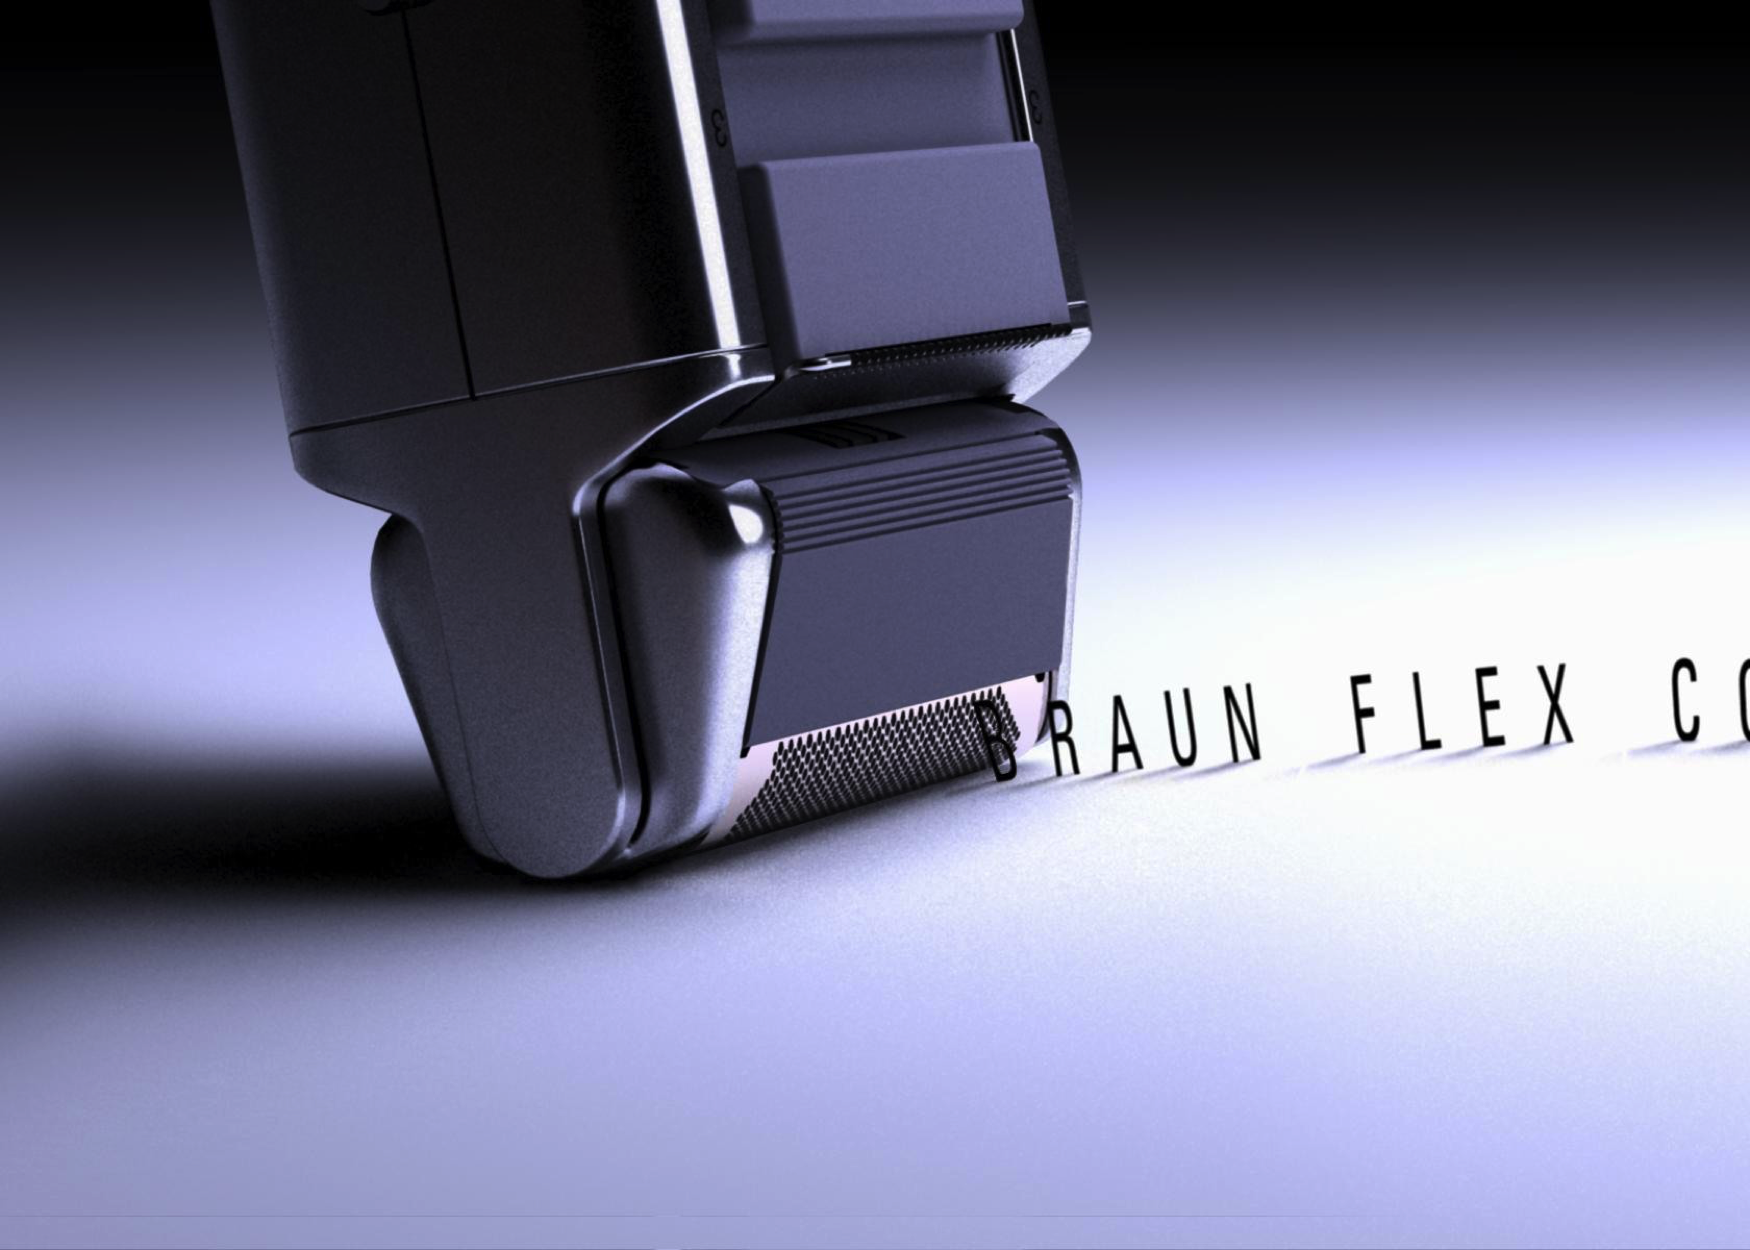
\includegraphics[width=\linewidth]{chap01/BraunRazor.png}
\end{marginfigure}
他们1998年上映的短片电影《棕兔夫人》\sidenote{译者注:Bunny。}
是在制作中使用蒙特卡洛全局照明的早期案例。
其视觉呈现与用Reyes渲染的电影和短片截然不同,获得了广泛关注。
蓝天工作室随后拍摄的故事片沿用了该方法。
不幸的是,蓝天工作室从未公开其方法的重要技术细节,限制了其扩大影响。

21世纪00年代初期,大量工作室使用主打视觉效果的\emph{mental ray}光线追踪渲染器系统。
它是实现了复杂全局光照算法的非常高效的光线追踪器。
其开发者主要关注计算机辅助设计和产品设计应用,
因此它缺乏电影制作所需的处理极其复杂场景和极多纹理贴图之类的特性。

《棕兔夫人》之后,2001年迎来了另一个分水岭,
Marcos Fajardo带着他早期版本的\emph{Arnold}渲染器来到了SIGGRAPH
\sidenote{译者注:即ACM Special Interest Group on Computer Graphics and Interactive Techniques,
    计算机图形学与交互技术特别兴趣小组,成立于1969年,其前身ACM SICGRAPH成立于1967年。}。
他展示了蒙特卡洛图像合成课程上的图片,
不仅有复杂几何体、纹理和全局光照,而且几十分钟内就能完成渲染。
尽管这些场景不如当时电影制作中用的那么复杂,
但他的结果证明了复杂场景中全局光照有许多创造性机会。

Fajardo把\emph{Arnold}带到了索尼影业图像工作室\sidenote{译者注:Sony Pictures Imageworks。},
开始将其转化为可用于制作的基于物理的渲染系统。
高效运动模糊、可编程着色、支持大量复杂场景和延迟加载场景体
以及在内存只保留一小部分场景纹理时支持纹理缓存等,这些都是需要解决的重要领域。
\emph{Arnold}在电影《怪兽屋》\sidenote{译者注:即Monster House,于2006年上映。}得到首次应用,
现在一般作为一款产品提供。

21世纪00年代中期,皮克斯\sidenote{译者注:即Pixar Animation Studios,皮克斯动画工作室,
    于1986年成立,
    % 前身为卢卡斯影业计算机部图形学小组(The Graphics Group of Lucasfilm Computer Division),
    代表作有
    《玩具总动员》(Toy Story)、
    《海底总动员》(Finding Nemo)、
    《超人总动员》(The Incredibles)、
    《赛车总动员》(Cars)、
    《机器人总动员》(WALL·E)、
    《飞屋环游记》(Up)、
    《头脑特工队》(Inside Out)、
    《心灵奇旅》(Soul)等。}的
\emph{RenderMan}渲染器开始支持混合栅格化和光线追踪算法
并包括了大量解决复杂场景下求解全局光照的创新算法。
\emph{RenderMan}最近遵循pbrt的一般系统架构\citep{10.1145/2776880.2792699}
\sidenote{译者注:此处参考文献笔者改为了同名同源发表但作者名单更全的文献。}
被重新编写为基于物理的光线追踪器。

基于物理的蒙特卡洛渲染方法成功用于制作的一大原因是
它们最终提高了艺术家们的生产力。
一些重要因素是:
\begin{itemize}
    \item 涉及的算法本质上只有一个质量旋钮:每个像素取多少次采样;
          这对艺术家们很有用。通过每个像素只采几个样本,
          光线追踪算法也适合渐进式改善和快速计算粗略预览图;
          基于栅格化的渲染器则没有等效功能。
    \item 采用基于物理的反射模型让设计表面材料变得简单。
          早前,当使用能量未必守恒的反射模型时,
          一个物体可能被放置在单光源环境下来调节其表面的反射参数。
          该物体在那个环境下可能看起来不错,
          但移到另一个光照环境时常常会显得完全不对,
          因为表面实际上反射了太少或太多的能量:
          表面属性被设为不合理的值。
    \item 光线追踪计算的阴影质量比栅格化方法好得多。
          取消微调阴影贴图分辨率、偏置以及其他参数的需求把灯光艺术家们的烦人任务消除了。
          此外,基于物理的方法本身还给他们带来了反射光和其他柔光效果,
          无需艺术手工调整过程。
\end{itemize}

在编写本书时,基于物理的渲染已广泛运用于计算机生成图像的电影制作当中;
\reffig{1.22}和\reffig{1.23}展示的图像就来自两部近年使用了基于物理方法的电影。
\begin{figure}[htbp]
    \centering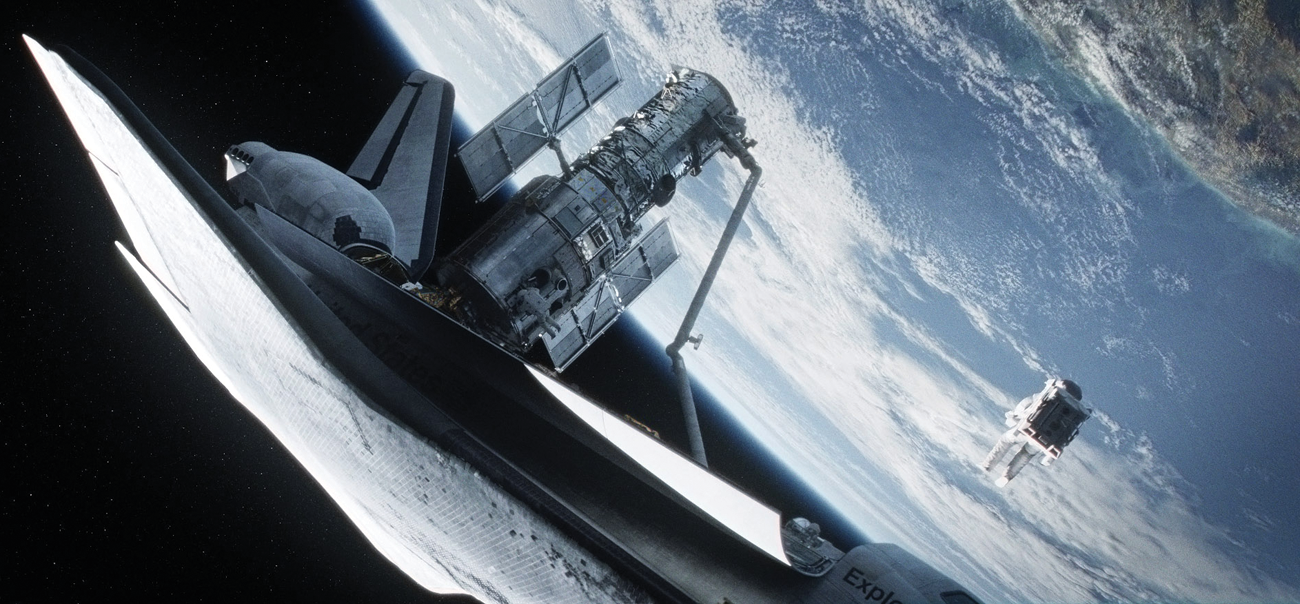
\includegraphics[width=\linewidth]{chap01/gravity.png}
    \caption{《地心引力》(Gravity, 2013)以计算机生成
        具备体积散射和大量各向异性金属表面的壮观逼真太空环境图像为特色。
        它由支持全局照明的基于物理的渲染系统\emph{Arnold}生成。
        该图由华纳兄弟(Warner Bros.)和Framestore提供。
    }
    \label{fig:1.22}
\end{figure}
\begin{figure}[htbp]
    \centering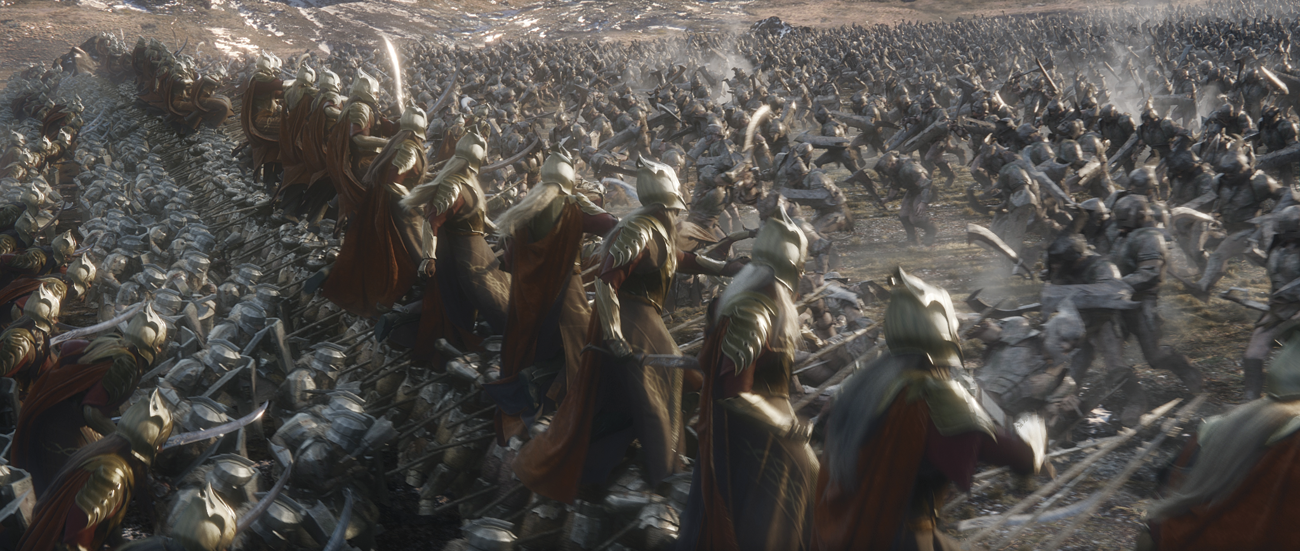
\includegraphics[width=\linewidth]{chap01/hobbit.png}
    \caption{来自《霍比特人3:五军之战》(The Hobbit: The Battle of the Five Armies, 2014)的
        该图也是用基于物理的渲染系统渲染得到的;
        这些角色以异质表面下的散射和大量几何细节为特点。
        图像由维塔数码(Weta Digital)制作,由华纳兄弟和米高梅(Metro-Goldwyn-Mayer)提供。}
    \label{fig:1.23}
\end{figure}
